\documentclass[10pt,twocolumn]{article}
\usepackage[a4paper,margin=0.65in,top=0.6in,bottom=0.6in]{geometry}
\usepackage{amsmath,amssymb}
\usepackage{graphicx}
\usepackage{booktabs}
\usepackage{hyperref}
\usepackage{titlesec}
\usepackage{caption}
\titlespacing*{\section}{0pt}{6pt}{3pt}
\titlespacing*{\subsection}{0pt}{4pt}{2pt}
\captionsetup{font=small,skip=3pt}
\setlength{\columnsep}{18pt}
\setlength{\parskip}{2pt}
\setlength{\abovedisplayskip}{3pt}
\setlength{\belowdisplayskip}{3pt}
\hypersetup{colorlinks=true,urlcolor=blue}

\title{\vspace{-14pt}\textbf{DamRL: Reservoir Release Control with Deep Q-Learning}\vspace{-6pt}}
\author{
  Nakshatra Cial (B24CM1090) \quad Harshita Pareek (B24CM1028)\\
  \small CSL3090 Artificial Intelligence, Assignment 2\\
  \small GitHub: \url{https://github.com/sudochill042/DamRL_CSL3090_A2_Mini_Project}
  \vspace{-10pt}
}
\date{}

\begin{document}
\maketitle

\section{Problem}
A reservoir operator decides every day how much water to release downstream. Releasing too little before the monsoon leaves no room for floods; releasing too much leaves shortages in the dry season. We model one year of daily operation of a single reservoir as a Markov decision process and train DQN and Double DQN agents on a synthetic simulator with stochastic inflows, an approach motivated by prior work on reinforcement learning for reservoir operation~\cite{wang2020,bertoni2020}. Agents are compared with fixed-release, greedy and seasonal rule-curve baselines, including on drought, extreme-flood and shifted-monsoon years that the agents never saw during training. All simulator constants are assumptions, kept in \texttt{configs/default.yaml}. Units are MCM (million cubic metres) and MCM/day.

\section{State Space}
The observation at day $t$ is a 10-dimensional vector, all entries scaled to roughly $[0,1]$:
\begin{align*}
s_t = \big[&\hat S_t,\ \sin\theta_t,\ \cos\theta_t,\ \tfrac{I_{t-1}}{30},\ \tfrac{\bar I_{7}}{30},\ \tfrac{D_t}{10},\\
           &\tfrac{R_{t-1}}{30},\ \tfrac{\tilde I_{t}}{30},\ \tfrac{\tilde I_{t+1}}{30},\ \tfrac{\tilde I_{t+2}}{30}\big]
\end{align*}
where $\hat S_t=(S_t-S_{\min})/(S_{\max}-S_{\min})$ is the storage fraction, $\theta_t=2\pi t/365$ encodes the season, $I_{t-1}$ is yesterday's inflow, $\bar I_7$ the 7-day mean inflow, $D_t$ today's demand, $R_{t-1}$ the previous release and $\tilde I_{t+k}$ a noisy inflow forecast with relative error $\sigma_k=0.15(k+1)$. The agent never sees the true inflow of the current day. Capacity $S_{\max}=1000$, dead storage $S_{\min}=100$, flood threshold $S_f=850$.

\section{Action Space}
Seven discrete release commands, $a\in\{0,5,10,15,20,25,30\}$ MCM/day. A command larger than the water available above dead storage is clipped and counted as a violation. An optional action mask removes commands that would breach dead storage even with zero inflow.

\section{Reward Function}
After the release the storage updates by mass balance,
$S_{t+1}=\min(S_{\max},\,S_t+I_t-R_t-E_t)$ with evaporation $E_t=0.0005\,S_t$ and spill $Q_t=\max(0,\,S_t+I_t-R_t-E_t-S_{\max})$. The daily reward is
\begin{align*}
r_t = &-w_s\,\tfrac{\max(0,D_t-R_t)}{10} - w_f\,\tfrac{\max(0,S_{t+1}-S_f)}{S_{\max}-S_f} \\
      &- w_d\,\tfrac{\max(0,R_t+Q_t-Q_{\text{safe}})}{R_{\max}} - w_c\,\mathbb{1}[\text{clip}] + w_p\,P_t
\end{align*}
with shortage, flood-pool, downstream-flow and clipping penalties and a hydropower proxy $P_t=\tfrac{R_t}{R_{\max}}\big(0.5+0.5\,\hat S_t\big)$ (release times head). Weights: $w_s=1,\ w_f=1,\ w_d=3,\ w_c=0.5,\ w_p=0.2$; $Q_{\text{safe}}=25$, $R_{\max}=30$. An episode is 365 days starting from storage $\sim U(450,650)$, discount $\gamma=0.99$.

\section{Environment and Algorithm}
\textbf{Inflow model.} Daily inflow is a seasonal mean (baseflow 4 plus a Gaussian monsoon bump of amplitude 26 centred on day 200) multiplied by lognormal noise with AR(1) persistence ($\phi=0.7$, $\sigma=0.5$), so wet and dry spells last several days. Demand is a cosine peaking in the dry season. Four scenarios: \emph{ordinary}; \emph{drought} (inflow $\times0.6$); \emph{extreme} (a 7-day wet spell followed by a 4-day pulse at $4\times$ inflow, random start between day 180 and 240); \emph{shifted} (monsoon centred on day 225, noisier). Agents are trained on ordinary years (or a 60/20/20 ordinary/drought/extreme mix) and tested on a frozen set of 250 seeded episodes (100 ordinary, 50 each drought, extreme, shifted). A separate frozen validation set of 90 episodes is used for model selection and baseline tuning.

\textbf{Baselines.} \emph{Random}; \emph{fixed} release of 10 MCM/day; \emph{greedy}, which releases the level nearest to demand and switches to maximum release once storage enters the flood pool; and a \emph{seasonal rule curve}, the standard operating rule of real reservoirs: a target storage $S^*(t)$ is a cosine between a low and high level, and the release is $D_t+g\,(S_t-S^*(t))/R_{\max}$ rounded to the nearest level. Its four parameters (low 200, high 500, lowest on day 150, gain 1) were grid-searched on the validation set.

\textbf{Algorithm.} DQN, introduced for deep reinforcement learning by Mnih et al.~\cite{mnih2015}, with an MLP Q-network ($10\to128\to128\to7$, ReLU), replay buffer of $10^5$ transitions, batch 128, Adam ($5\times10^{-4}$), Huber loss, target network copied every 1000 steps, $\epsilon$ decayed linearly from 1 to 0.05 over the first 60\% of training. Double DQN uses the online network to choose $a'$ and the target network to evaluate it, following van Hasselt et al.~\cite{vanhasselt2016}. Each agent is trained for 300 episodes ($\approx1.1\times10^5$ steps, about 15 minutes on CPU) with three seeds; the checkpoint with the best validation return is kept. DQN was chosen because the action space is small and discrete and the problem is a standard episodic MDP, so a value-based method is a natural fit; Double DQN tests whether overestimation matters here.

\section{Results}
\begin{table}[h]
\centering\footnotesize
\setlength{\tabcolsep}{3.5pt}
\caption{Mean per-episode metrics over 250 test years (agents: mean of seeds). CI is the 95\% interval over the 250 test episodes, seeds averaged per episode first; Short.\ is total shortage (MCM); Flood and Clip are days per year.}
\label{tab:main}
\begin{tabular}{lrrrrr}
\toprule
Method & Return $\pm$CI & Short. & Spill & Flood & Clip\\
\midrule
Random        & $-196.4\pm4.6$ & 1058 & 172 & 30.1 & 127.9\\
Fixed 10      & $-143.3\pm4.5$ &  447 & 457 & 70.2 &  82.9\\
Greedy        & $-102.1\pm3.7$ &  543 &  76 & 30.6 &  61.7\\
Rule curve    &  $-49.9\pm3.6$ &  531 &  43 & 11.5 &   2.1\\
DQN           &  $-37.9\pm3.4$ &  456 &  41 &  7.6 &   2.3\\
Double DQN    &  $-36.2\pm3.2$ &  447 &  38 &  6.7 &   1.3\\
DQN mixed     &  $-36.5\pm3.0$    & 451 & 43 & 7.7 & 0.1\\
DQN masked    &  $-40.3\pm3.6$     & 506 & 32 & 5.8 & 0.0\\
\bottomrule
\end{tabular}
\end{table}

\begin{table}[h]
\centering\footnotesize
\caption{Mean test return per scenario. Agents were trained on ordinary years only (except DQN mixed).}
\label{tab:scen}
\begin{tabular}{lrrrr}
\toprule
Method & Ordinary & Drought & Extreme & Shifted\\
\midrule
Rule curve  & $-29.5$ & $-78.9$ & $-57.9$ & $-53.5$\\
DQN         & $-17.7$ & $-71.7$ & $-40.0$ & $-42.6$\\
Double DQN  & $-17.5$ & $-69.4$ & $-37.0$ & $-39.4$\\
DQN mixed   & $-19.3$ & $-60.9$ & $-42.2$ & $-40.9$\\
DQN masked  & $-19.9$ & $-82.3$ & $-37.5$ & $-42.0$\\
\bottomrule
\end{tabular}
\end{table}

\begin{figure*}[t]
\centering
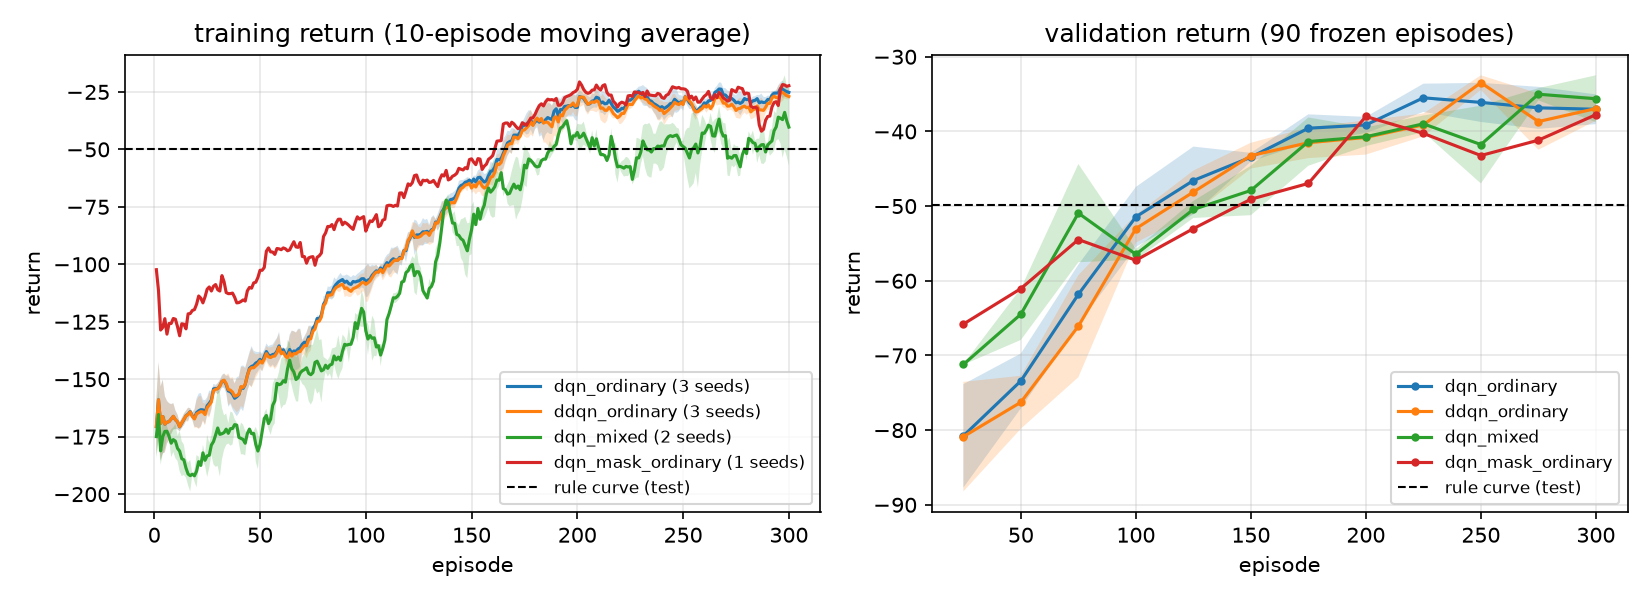
\includegraphics[width=0.85\textwidth]{../results/figures/learning_curves_report.png}
\caption{Training return (10-episode moving average) and validation return, mean $\pm$ std over seeds. Dashed line: rule curve on the test set.}
\label{fig:lc}
\end{figure*}

\begin{figure*}[t]
\centering
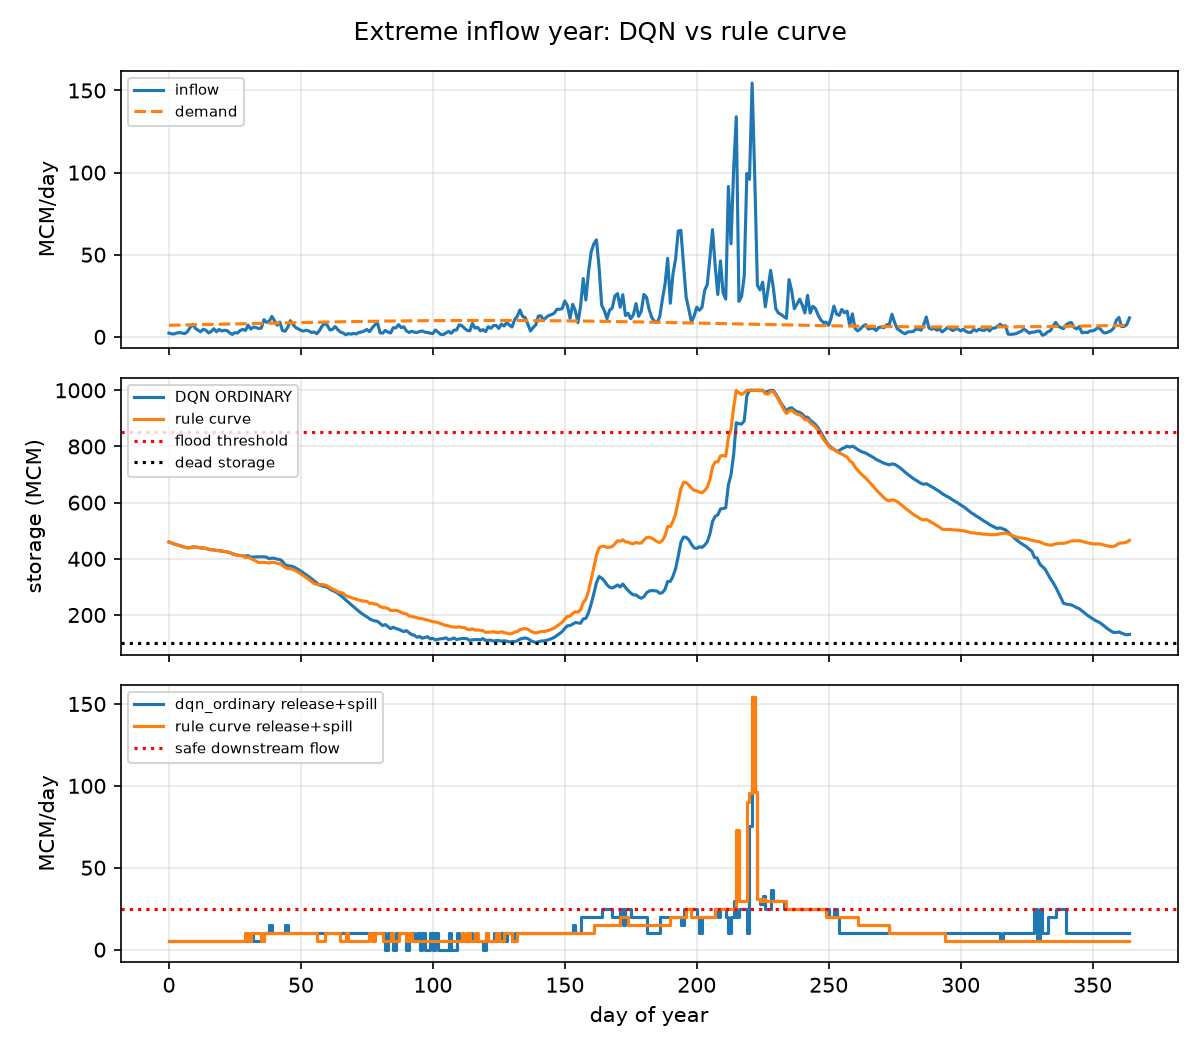
\includegraphics[width=0.85\textwidth]{../results/figures/trajectory_extreme.png}
\caption{One extreme test year. DQN keeps storage lower through the early monsoon (days 160 to 215) so the reservoir fills later and spills less; both methods spill during the 150 MCM/day pulse. The drawdown after day 300 is a finite-horizon effect: water has no value after day 365.}
\label{fig:traj}
\end{figure*}

Both agents beat every baseline on every scenario (Tables~\ref{tab:main}, \ref{tab:scen}). Against the tuned rule curve, DQN improves the return by 24\%, cuts flood-pool days from 11.5 to 7.6 and downstream violations from 5.5 to 2.3 days per year, with 14\% less total shortage. The learning curves (Fig.~\ref{fig:lc}) rise past the rule curve after about 150 episodes and the three seeds agree within a few units of return. Double DQN is slightly better than DQN ($-36.2$ vs $-37.9$) but the confidence intervals overlap, so with only seven actions overestimation is not a major issue here. The agents trained only on ordinary years still transfer to drought, extreme and shifted years, mainly because the state includes the storage fraction, season and short forecast, which is enough to react to unusual inflow. Training on the 60/20/20 scenario mix (DQN mixed, 2 seeds) gives the same overall return but improves drought years the most ($-60.9$ vs $-71.7$) at a small cost on ordinary and extreme years, so seeing dry years in training teaches the agent to save water. Action masking (1 seed; releases larger than the water above dead storage are removed from the argmax, using observed storage only) removes clipping entirely and gives the fewest flood days, but the masked agent holds back too much water, has the largest shortage and the lowest return of the agents ($-40.3$), so the clipping penalty alone is a better teacher than a hard mask here. Fig.~\ref{fig:traj} shows the learned behaviour: the agent runs the reservoir close to dead storage before the monsoon and delays filling during the early monsoon, which the rule curve cannot do because it tracks a fixed target, so it has more room when the flood pulse arrives.

\textbf{Failure cases.} Four of the five worst DQN test episodes are extreme years with 470 to 910 MCM of spill and 35 to 57 flood-pool days: the flood pulse (over 100 MCM/day for several days) arrives when storage is already high, and the 30 MCM/day outlet cannot drain the reservoir fast enough, so spill is physically unavoidable and every method suffers. The fifth is a drought year in which the agent reaches dead storage and records 241 shortage days. The hydropower term rewards release, so the agent has little reason to save water for a drought it is not told is coming.

\section{Conclusion}
A DQN agent with a compact state (storage, season, recent and forecast inflow, demand) learns a release policy that outperforms a tuned seasonal rule curve by about 24\% in return and cuts flood-pool days by a third, and it generalises to inflow regimes it never trained on. Double DQN gives a small, not significant, further gain. Limitations: the simulator is synthetic, hydropower is a crude proxy, and the agent cannot avoid spill when a large pulse hits a full reservoir or shortage in a long drought. Even so, the problem is a real one: Indian reservoirs are operated every day on rule curves like our baseline, and monsoon floods and dry-season shortages are the exact trade-off the reward encodes. The simulator is synthetic, but the pipeline is what a real deployment needs: the state, reward and scenario tests carry over unchanged, and the inflow generator can be replaced by historical gauge data for a specific dam. In practice the agent would act as decision support, suggesting a daily release that the operator can accept or override, with the rule curve as a fallback.

\begin{thebibliography}{9}
\small

\bibitem{wang2020}
X. Wang et al.,
``Efficient Reservoir Management through Deep Reinforcement Learning,''
AI for Earth Sciences Workshop at NeurIPS, 2020.
Available: \url{https://arxiv.org/abs/2012.03822}.

\bibitem{masoumi2025}
F. Masoumi, M. Jorabloo, and G. Shobeyri,
``Optimizing Reservoir Operations with Reinforcement Learning:
A Data-Driven Framework,''
\textit{Civil Engineering and Applied Solutions},
vol. 1, no. 4, pp. 56--67, 2025.
Available: \href{https://www.magiran.com/paper/2894898/optimizing-reservoir-operations-with-reinforcement-learning-a-data-driven-framework?lang=en}{[Optimizing Reservoir Operations with Reinforcement Learning:
A Data-Driven Framework]}.

\bibitem{bertoni2020}
F. Bertoni, M. Giuliani, and A. Castelletti,
``Integrated Design of Dam Size and Operations via Reinforcement Learning,''
\textit{Journal of Water Resources Planning and Management},
vol. 146, no. 4, 2020.
Available: \url{https://doi.org/10.1061/(ASCE)WR.1943-5452.0001182}.

\bibitem{mnih2015}
V. Mnih et al.,
``Human-level control through deep reinforcement learning,''
\textit{Nature}, vol. 518, pp. 529--533, 2015.
Available: \url{https://doi.org/10.1038/nature14236}.

\bibitem{vanhasselt2016}
H. van Hasselt, A. Guez, and D. Silver,
``Deep Reinforcement Learning with Double Q-Learning,''
Proceedings of the AAAI Conference on Artificial Intelligence,
vol. 30, no. 1, 2016.
Available: \url{https://doi.org/10.1609/aaai.v30i1.10295}.

\end{thebibliography}

\end{document}